The NeXus Constructor is a tool written with \textit{Qt for Python} that provides an interface for scientists to write, edit, and examine NeXus files. \iffalse Such files can then be used for configuring the experiment control software in order to write real-time data. \fi The NeXus Constructor has the a number of key features:

% Someone may not know what experiment control software does, what makes real-time data good, etc.

\begin{itemize}
\setlength\itemsep{1.1em}
\item Instrument View - A Qt3D pane that draws the experiment components in 3D.
\item Component List - A list of the components contained in the NeXus file.
\item Add Component Dialog - A tool with which users can add components to a NeXus file.
\item NeXus File Layout - An illustration of the hierarchical NeXus structure.
\end{itemize}

\begin{figure}
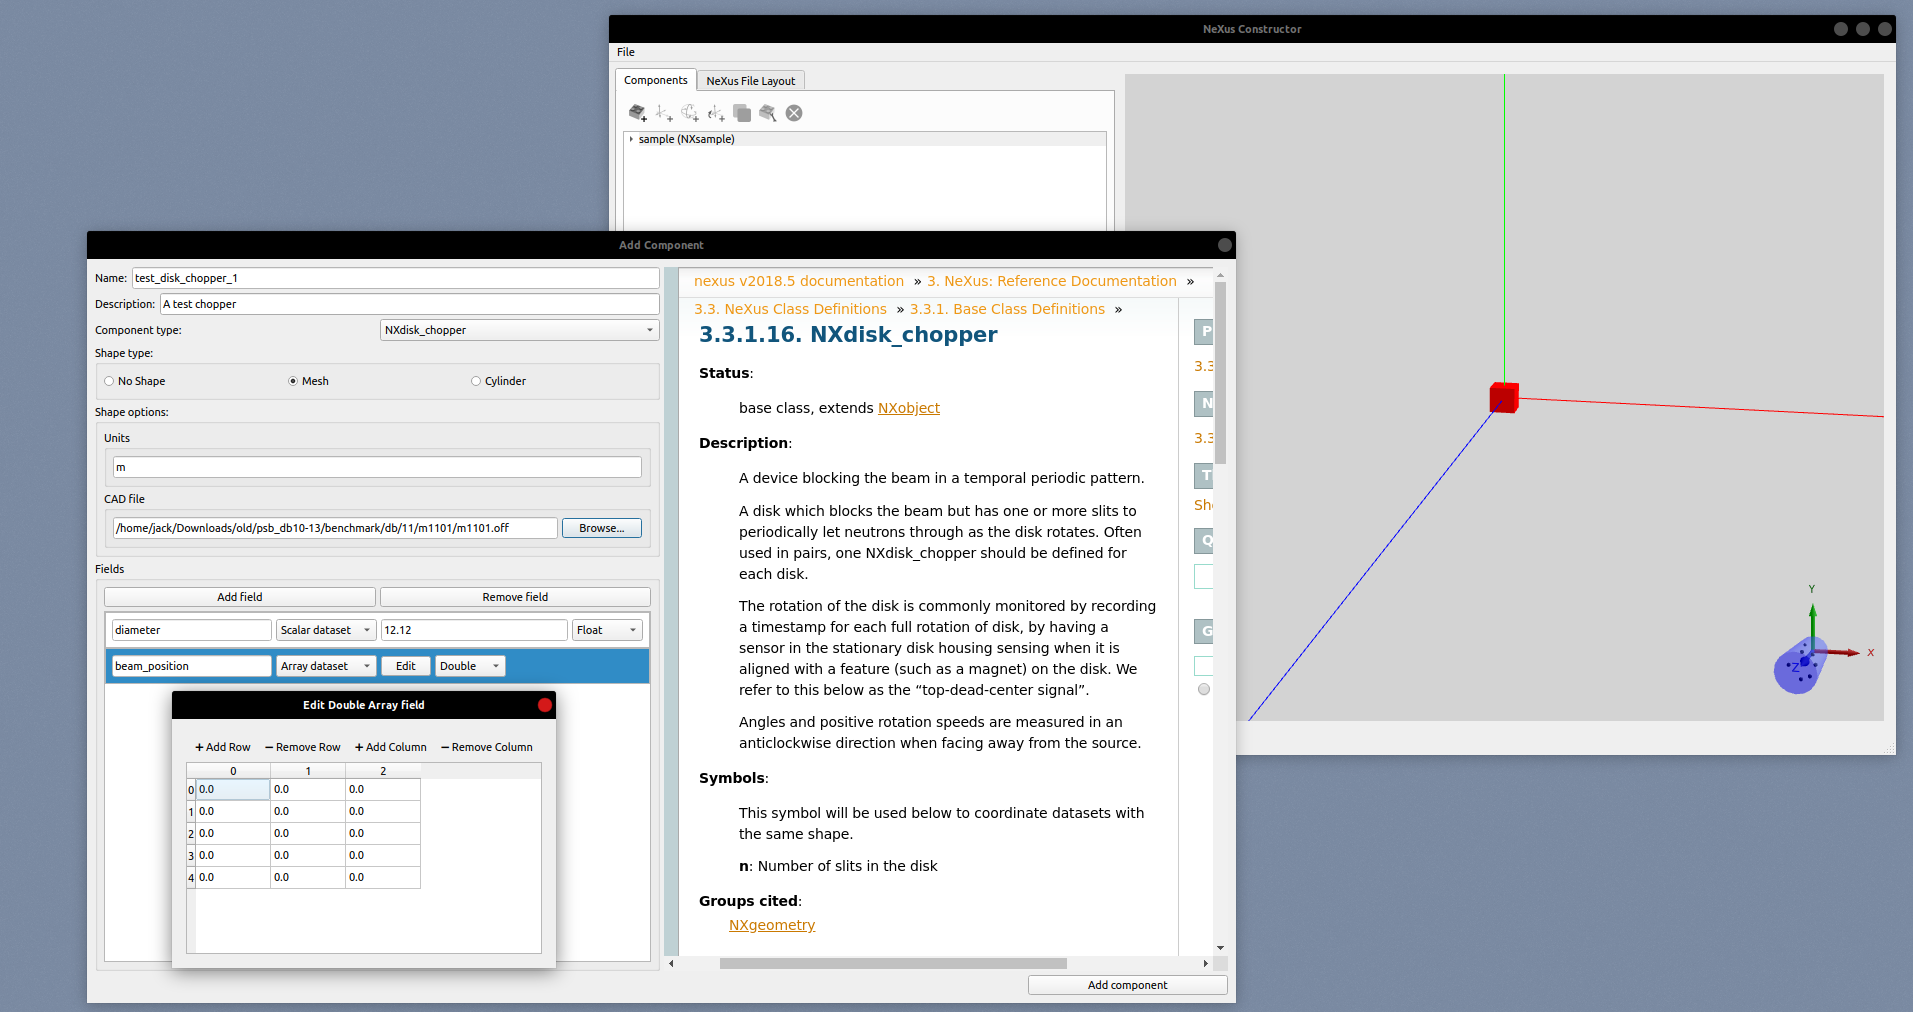
\includegraphics[width=\linewidth]{screenshot.png}
\caption{Screenshot of the NeXus Constructor. The file that is open in the NeXus Constructor contains a single component, an \texttt{NX\_sample}, which is represented by a red cube in the main window's Instrument View. In front of the main window is the Add Component Dialog through which users can add components to their NeXus file. In this example the Add Component Dialog is being used to create a \texttt{NXdisk\_chopper} component.}
\end{figure}
\iffalse
% Other Advantages of Using the NeXus Constructor
\begin{itemize}
    \item Being able to visualise components helps users detect errors. 
    \item The creation of components can be performed in a ``smart" way. The application can determine what fields need to be completed in order to create a component of a particular class. 
    \item Verification can take place as a user enters information into a NeXus file. Adding information that does not align with certain requirements is prohibited.
\end{itemize}
\fi
